\section{Using Project-Join Trees for Weighted Model Counting}
\label{sec_jointree}

In model counting, a Boolean formula is often given in conjunctive normal form (CNF), \ie, as a set $\phi$ of clauses.
For each clause $c \in \phi$, define $\vars(c)$ to be the set of variables appearing in $c$.
Then $c$ represents a Boolean function over $\vars(c)$. Similarly, $\phi$ represents a Boolean function over $\vars(\phi) \equiv \bigcup_{c \in \phi} \vars(c)$. 

It is well-known that weighted model counting can be performed through a sequence of projections and joins on pseudo-Boolean functions \cite{DPV20,DDV19}.
Given a CNF formula $\phi$ and a literal-weight function $W$ over a set $X$ of variables, the corresponding weighted model count can be computed as follows:
\begin{equation}
\label{eq_factored_wmc}
    W(\phi) = \pars{
        % \proj_{x_1} \cdots \proj_{x_n}
        \proj_X
        \pars{\prod_{c \in \phi} c \mult \prod_{x \in X} W_x}
    }(\emptyset)
\end{equation}

By taking advantage of the associative and commutative properties of multiplication as well as the commutative property of projection, we can rearrange Equation \eqref{eq_factored_wmc} to apply early projection.
It was shown in \cite{DPV20} that early projection can significantly reduce computational cost.
There are a variety of possible rearrangements of Equation \eqref{eq_factored_wmc} of varying costs.
Although \cite{DPV20} considered several heuristics for performing this rearrangement (using bucket elimination \cite{dechter99} and Bouquet's Method \cite{bouquet1999gestion}), they did not attempt to analyze rearrangements.

In this work, we aim to analyze the quality of the rearrangement, in isolation from the underlying implementation and data structure used for Equation \eqref{eq_factored_wmc}.
This approach has been highly successful for database-query optimization \cite{MPPV04}, where the central object of theoretical reasoning is the \emph{query plan}.
The approach has also seen similar success in Bayesian network inference \cite{darwiche1998dynamic}.

We model a rearrangement of Equation \eqref{eq_factored_wmc} as a \emph{project-join tree}:
\begin{definition}[Project-Join Tree]
\label{def_jointree}
    Let $X$ be a set of Boolean variables and $\phi$ be a CNF formula over $X$.
    A \emph{project-join tree} of $\phi$ is a tuple $(T, r, \gamma, \pi)$ where:
    \begin{itemize}
        \item $T$ is a tree with root $r \in \V{T}$,
        \item $\gamma: \Lv{T} \to \phi$ is a bijection between the leaves of $T$ and the clauses of $\phi$, and
        \item $\pi: \V{T} \setminus \Lv{T} \to 2^X$ is a labeling function on internal nodes.
    \end{itemize}
    Moreover, $(T, r, \gamma, \pi)$ must satisfy the following two properties:
    \begin{enumerate}[ref=\arabic*]
        \item $\{\pi(n) : n \in \V{T} \setminus \Lv{T} \}$ is a partition of $X$, and \label{prop1}
        \item for each internal node $n \in \V{T} \setminus \Lv{T}$, variable $x \in \pi(n)$, and clause $c \in \phi$ \st{} $x$ appears in $c$, the leaf node $\gamma^{-1}(c)$ must be a descendant of $n$ in $T$. \label{prop2}
    \end{enumerate}
\end{definition}
If $n$ is a leaf node, then $n$ corresponds to a clause $c = \gamma(n)$ in Equation \eqref{eq_factored_wmc}.
If $n$ is an internal node, then $n$'s children $\C{T}{r}{n}$ are to be multiplied before the projections of variables in $\pi(n)$ are performed.
The two properties ensure that the resulting expression is equivalent to Equation \eqref{eq_factored_wmc} using early projection.
See Figure \ref{fig_join_tree} for a graphical example of a project-join tree.
\begin{figure}%[H]
    \centering
    \begin{tikzpicture}[grow=right] % use '~' for space; ' ' would crash
        \tikzset{level distance=80pt,sibling distance=-6pt}
        \tikzset{execute at begin node=\strut}
        \tikzset{every tree node/.style={anchor=base west}}
        \Tree [ .$n_{8}\piMap\emptyset$
            [ .$n_{7}\piMap\set{x_3, x_4}$
                [ .$n_{6}\piMap\set{x_1}$
                    [ .$n_4\gammaMap{x_1 \vee x_3 \vee \neg x_4}$ ]
                    [ .$n_3\gammaMap{\neg x_1 \vee \neg x_3}$ ]
                ]
                [ .$n_2\gammaMap{x_3 \vee x_4}$ ]
            ]
            [ .$n_{5}\piMap\set{x_2}$ [ .$n_1\gammaMap{\neg x_2}$ ] ]
        ]
    \end{tikzpicture}
\caption{
    A project-join tree $(T, n_{8}, \gamma, \pi)$ of a CNF formula $\phi$.
    Each leaf node is labeled by $\gamma$ with a clause of $\phi$.
    Each internal node is labeled by $\pi$ with a set of variables of $\phi$.
}
\label{fig_join_tree}
\end{figure}

Project-join trees have previously been studied in the context of database-query optimization \cite{MPPV04}.
Project-join trees are closely related to contraction trees in the context of tensor networks \cite{EP14,DDV19}.
Once a rearrangement of Equation \eqref{eq_factored_wmc} has been represented by a project-join tree, we can model the computation process according to the rearrangement.
In particular, given a literal-weight function $W = \prod_{x \in X} W_x$, we define the $W$-\emph{valuation} of each node $n \in \V{T}$ as a pseudo-Boolean function associated with $n$.
The $W$-valuation of a node $n \in \V{T}$ is denoted $f^W_n$ and defined as follows:
\begin{equation}
\label{eq_valuation}
    f^W_n \equiv
    \begin{cases}
       \gamma(n) & \text{if}~n \in \Lv{T} \\
        \sum_{\pi(n)} \pars{ \prod_{o \in \C{T}{r}{n}} f^W_o \cdot \prod_{x \in \pi(n)} W_x } & \text{if}~n \notin \Lv{T}
    \end{cases}
\end{equation}

Note that the $W$-valuation of a leaf node $n \in \Lv{T}$ is a clause $c = \gamma(n) \in \phi$, interpreted in this context as an associated function $\lambda_c : 2^{\vars(c)} \to \B$ where $\lambda_c(\tau) = 1$ if and only if the truth assignment $\tau$ satisfies $c$.
The main idea is that the $W$-valuation at each node of $T$ is a pseudo-Boolean function computed as a subexpression of Equation \eqref{eq_factored_wmc}.
The $W$-valuation of the root is exactly the result of Equation \eqref{eq_factored_wmc}, \ie, the weighted model count of $\phi$ \wrt{} $W$:
\begin{theorem}
\label{thm_valuation_wmc}
    Let $\phi$ be a CNF formula over a set $X$ of variables, $(T, r, \gamma, \pi)$ be a project-join tree of $\phi$, and $W$ be a literal-weight function over $X$.
    Then $f^W_r(\emptyset) = W(\phi)$.
\end{theorem}

This gives us a two-phase algorithm for computing the weighted model count of a formula $\phi$.
First, in the \emph{planning} phase, we construct a project-join tree $(T, r, \gamma, \pi)$ of $\phi$.
We discuss algorithms for constructing project-join trees in Section \ref{sec_planning}.
Second, in the \emph{execution} phase, we compute $f^W_r$ by following Equation \eqref{eq_valuation}.
We discuss data structures for computing Equation \eqref{eq_valuation} in Section \ref{sec_execution}.

When computing a $W$-valuation, the number of variables that appear in each intermediate pseudo-Boolean function has a significant impact on the runtime.
The set of variables that appear in the $W$-valuation of a node is actually independent of $W$.
In particular, for each node $n \in \V{T}$, define $\vars(n)$ as follows:
\begin{equation}
    \vars(n) \equiv
    \begin{cases}
        \vars(\gamma(n)) & \text{if}~n \in \Lv{T} \\
        \pars{\bigcup_{o \in \C{T}{r}{n}} \vars(o)} \setminus \pi(n) & \text{if}~n \notin \Lv{T}
    \end{cases}
\end{equation}

For every literal-weight function $W$, the domain of the function $f^W_n$ is $2^{\vars(n)}$.
To characterize the difficulty of $W$-valuation, we define the \emph{size} of a node $n$, $\func{size}(n)$, to be $\size{\vars(n)}$ for leaf nodes and $\size{\vars(n) \cup \pi(n)}$ for internal nodes.
The \emph{width} of a project-join tree $(T, r, \gamma, \pi)$ is $\func{width}(T) \equiv \max_{n \in \V T} \func{size}(n)$.
We see in Section \ref{sec_experiments} how the width impacts the computation of $W$-valuations.

% Project-join trees are related to \emph{variable elimination} on factor graphs \cite{KDLD05,BDP09}, which uses tree decompositions of the primal graph of a factor graph.

% To do this, we separate the algorithm of \cite{DPV20} into two phases.
% First, in the \emph{planning} phase, we produce a rearrangement of Equation \eqref{eq_factored_wmc}.
% Second, we construct a project-join tree $(T, r, \gamma, \pi)$ of $\phi$.
% We discuss algorithms for constructing project-join trees in Section \ref{sec_planning}.
% Second, in the \emph{execution} phase, compute $f^W_r$ by following Equation \eqref{eq_valuation}.

% Although \cite{DPV20} considered various heuristics for performing this rearrangement (using bucket elimination \cite{dechter99} and Bouquet's Method \cite{bouquet1999gestion}), they did not specifically analyze the quality of the rearrangement is isolation from the underlying data structures.

% As noted in Section \ref{sec_prelim}, if $\phi: 2^X \to \{0,1\}$ is a Boolean formula and $W: 2^X \to \R$ is a pseudo-Boolean function, then $W(\phi) = \left(\sum_X (\phi \mult W) \right)(\emptyset)$.
% Moreover, \cite{DPV20} observed that, $\phi$ and $W$ can both be given in factored forms $\phi = \prod_{C_i} C_i$ (\ie, as a set of clauses) and $W = \prod_{x \in X}$ (\ie, as a literal-weight function).

% In this section, we define a project-join tree.
% We then show how a project-join tree can be used to perform weighted model counting.

% Given a CNF formula, we can construct a project-join tree, which specifies an order to apply projection and multiplication operations for model counting.

% For a project-join tree $(T, r, \gamma, \pi)$, the structure of $T$ indicates the order that multiplication should occur between the clauses at each leaf, while $\pi$ indicates the variable projections that should occur after each multiplication.
